\chapter{Apéndice C: Esquemático completo del circuito resonante en serie} % Título centrado y en negrita según norma
\addcontentsline{toc}{chapter}{Apéndice C: Esquemático del circuito}
\label{ape:esquematico}

% Usamos sidewaysfigure para que el esquema se vea en horizontal y sea legible
\begin{sidewaysfigure}[htbp]
    \centering
    % Ajusta el width al 1.0 para que use todo el ancho de la página tabloide/carta
    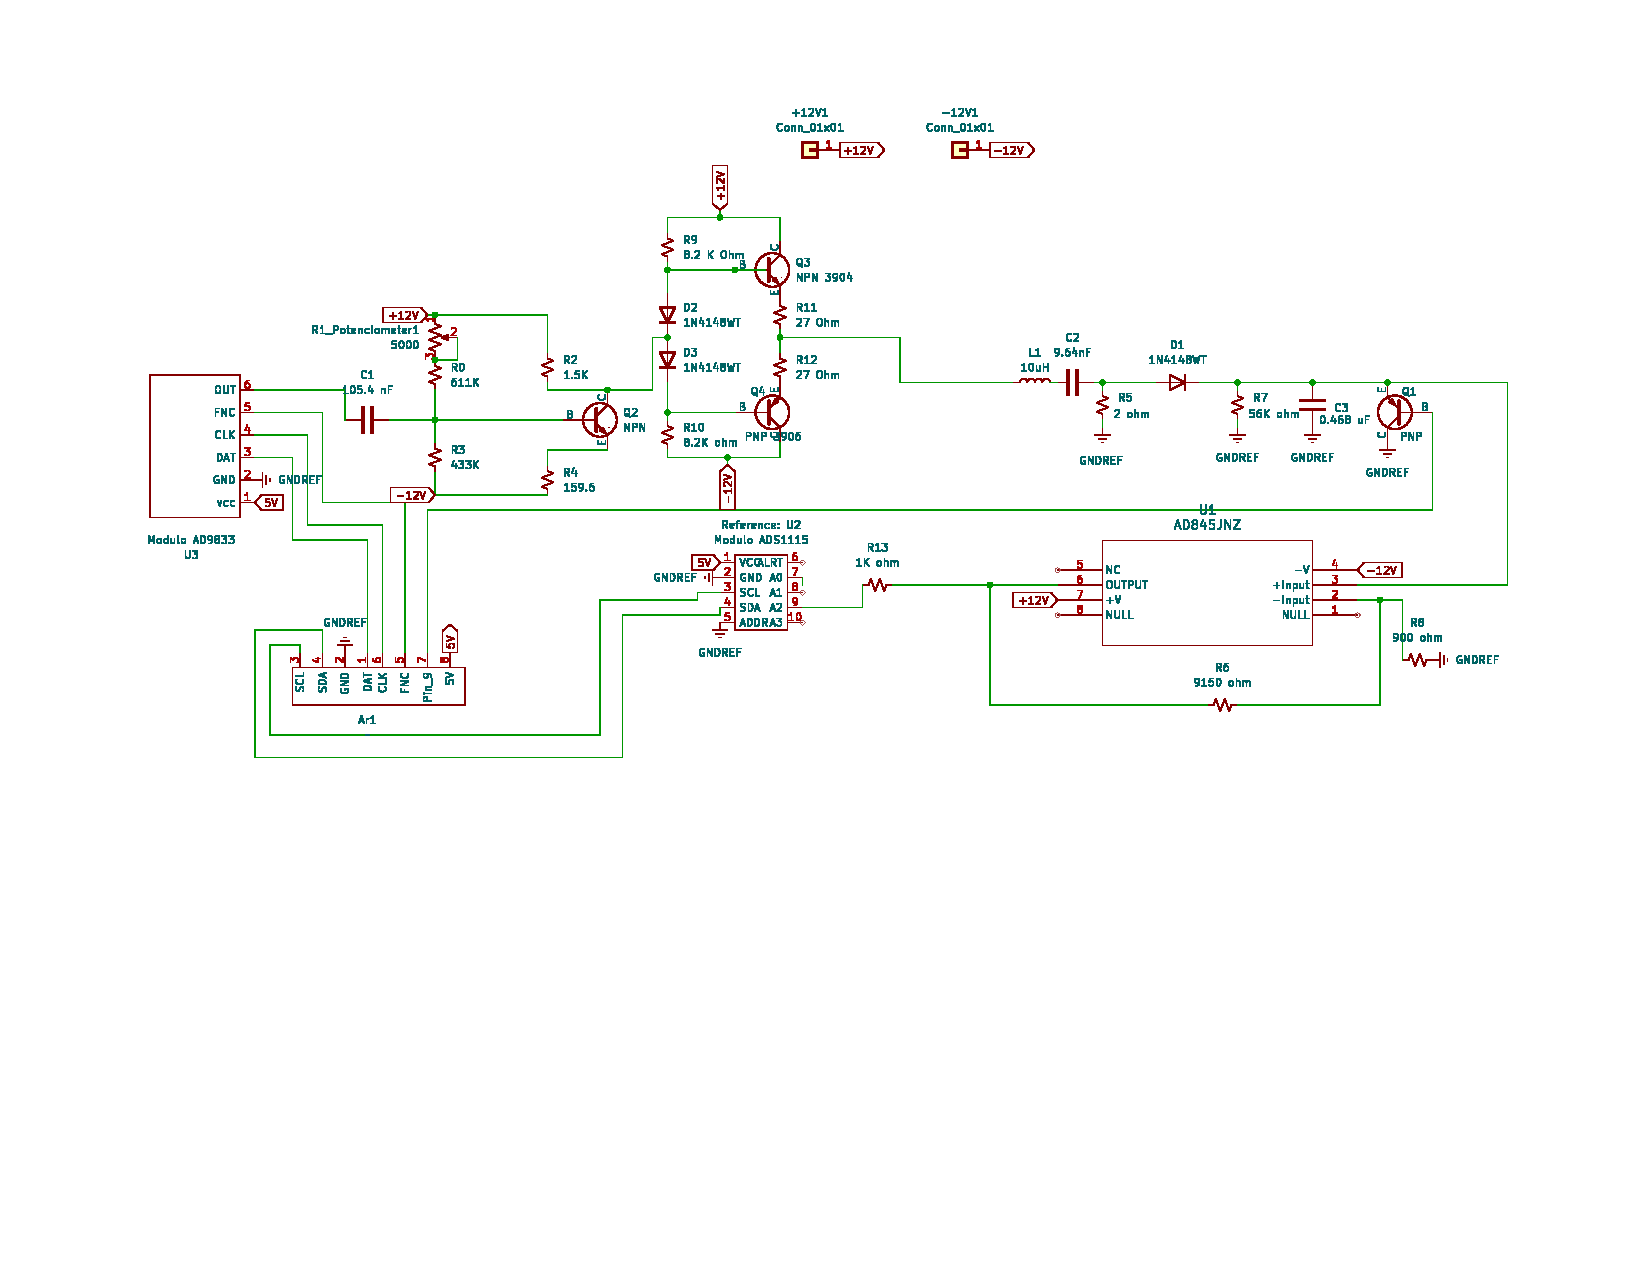
\includegraphics[width=1.0\linewidth]{esquematico-kidcad-final.pdf}
    
    \vspace{1em} % Espacio entre imagen y título
    
    % Título centrado y debajo (formato regular sin negritas según norma USB)
    \caption{Diagrama esquemático completo del prototipo conectado en serie diseñado en KiCad.}
    \label{fig:esquema_completo}
\end{sidewaysfigure}


